\chapter{Methods}\label{ch:methods}

This chapter describes the design of the hybrid reconstruction pipeline:
the property graph schema that stores the static artefacts, the separate
trace-collection pipeline, the agent skill architecture that can optionally be used to orchestrate
extraction and generation, the pattern-based instrumentation tool used for
trace collection, the scenario-scoped querying and Neo4j-based reachability filter that
produces scenario-specific interaction models.

\section{Pipeline Overview}\label{sec:pipeline-overview}

The pipeline takes a \Cpp\ source tree and, optionally, a set of
timestamped execution traces, and produces \sysml sequence diagrams
scoped to a user-specified scenario. It runs as four phases
(\cref{fig:pipeline-overview}). All four phases follow a fixed, deterministic rule set
given their inputs.

\begin{figure}[htb]
\centering
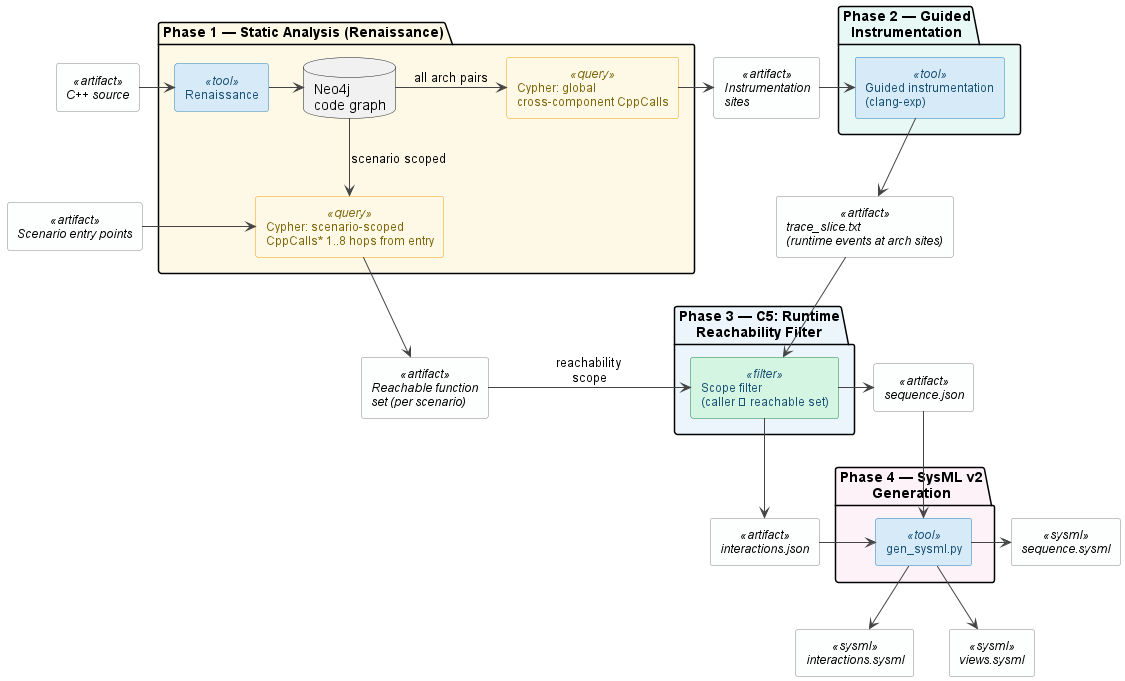
\includegraphics[width=1.2\textwidth, height=2\textheight, keepaspectratio]{figures/h1-full-pipeline_v1.png}
\caption{The concrete C5 pipeline as run for the H1 experiments, with
  the actual tools and artefacts behind each stage: Renaissance
  populating the \neo code graph and computing a scenario-scoped
  reachable function set via \texttt{CppCalls*1..8} traversal
  (Phase~1); guided instrumentation producing
  \texttt{trace\_slice.txt} at architecture-level call sites
  (Phase~2); the Neo4j-based reachability filter scoping
  \texttt{trace\_slice.txt} to callers in the reachable function set
  and writing \texttt{interactions.json} and \texttt{sequence.json}
  (Phase~3, condition~C5); and \texttt{gen\_sysml.py} rendering the
  final \sysml v2 output (Phase~4,
  \cref{sec:evidence-synthesis,sec:sysml-generation}).}
\label{fig:pipeline-overview}
\end{figure}

\begin{enumerate}
  \item \textbf{Phase~1 --- Static Analysis (Renaissance)}
    (\cref{sec:static-impl}). Renaissance analyses the \Cpp\ source and
    populates the \neo graph with 11 node labels and 11 relationship
    types (\cref{sec:pg-schema}); the CPSCore graph contains 67,104
    nodes. Two Cypher queries then run against the live graph: a
    scenario-scoped forward traversal (\texttt{CppCalls*1..8} from the
    scenario's entry-point functions) producing the
    \emph{reachable function set} consumed by Phase~3
    (\cref{sec:scoping-impl,sec:evidence-synthesis}), and a global
    cross-component query producing the architectural interface map
    identifying call sites eligible for instrumentation
    (\cref{sec:csp-matcher}). The scenario-scoped subgraph is also
    flattened into an ordered CSV table (condition~C2 static edge set,
    \cref{sec:h1-results}) via \texttt{get-interface-dependency-table}
    and \texttt{get-sequence-dependency-table}.

  \item \textbf{Phase~2 --- Guided Instrumentation}
    (\texttt{add-runtime-instrumentation}, \cref{sec:csp-matcher}).
    Pattern-based code transformation injects trace probes at the call
    sites identified in Phase~1; the instrumented binary is rebuilt and
    run, producing \texttt{trace\_slice.txt}.

  \item \textbf{Phase~3 --- C5: Neo4j-Based Reachability Filter}
    (\texttt{synthesis}, \cref{sec:evidence-synthesis}).
    \texttt{trace\_slice.txt} is filtered to events whose caller is in
    the Phase~1 reachable function set, removing setup-phase boilerplate
    and producing \texttt{interactions.json} and \texttt{sequence.json}.

  \item \textbf{Phase~4 --- SysML v2 Generation}
    (\texttt{draw-sysml-sequence-model},
    \texttt{draw-sysml-structural-model}, \cref{sec:sysml-generation}).
    \texttt{interactions.json} and \texttt{sequence.json} are projected
    into \sysml textual notation.
\end{enumerate}

Two further skills, \texttt{draw-sequential-mermaid-general} and
\texttt{draw-structural-mermaid}, offer a Mermaid-syntax visualisation of
the same reconstruction; they read the Phase~1 dependency tables directly
and are not part of this four-phase pipeline, since they bypass the
reachability filter rather than consuming its output.

Each skill is stateless and read-only with respect to the graph, except
the instrumentation skill, which modifies source files. Every skill
accepts a natural-language prompt and returns a structured artefact (CSV,
Cypher query, or model file), which allows the chain to be reused on a
new codebase without code changes.

\section{Property Graph Schema}\label{sec:pg-schema}

\subsection{Design Decision}\label{sec:pg-decision}

A \ac{PG} in \neo was chosen for the static knowledge store over a
relational database, a document store, and an in-memory graph library.
The pipeline traverses function$\to$file$\to$folder paths,
function$\to$function call chains, and class$\to$function containment
within the same query. The static graph can also be re-derived or extended without disturbing
the separate trace pipeline, since static edges are typed and
distinguishable from anything added later, and Cypher's pattern-matching
syntax maps directly onto the \texttt{text-to-cypher} skill
(\cref{sec:skill-design}): a natural-language scenario query becomes a
graph pattern with little translation. An in-memory graph library would
satisfy traversal alone, and a document store neither traversal nor
declarative querying.

\subsection{Node Types}\label{sec:node-types}

\Cref{tab:node-types} lists the 11 node labels emitted by Renaissance.

\begin{table}[htb]
\centering
\caption{Property graph node labels relevant to reconstruction. Each C++
  node (the \texttt{Cpp*} labels) carries \texttt{name}, \texttt{symbol}, \texttt{type}, and
  \texttt{lineNumber} properties}
\label{tab:node-types}
\small
\begin{tabular}{@{} l p{9cm} @{}}
\toprule
\textbf{Label} & \textbf{Semantics} \\
\midrule
\texttt{CppDeclaration}           & Class, struct, enum, or typedef declaration \\
\texttt{CppForwardDeclaration}    & Forward declaration of a class or struct \\
\texttt{CppFunctionDeclaration}   & Function prototype (header) \\
\texttt{CppFunctionDefinition}    & Function body (implementation) \\
\texttt{CppMacroDefinition}       & Preprocessor macro definition \\
\texttt{HeaderFile}               & \texttt{.h}/\texttt{.hpp} file \\
\texttt{SourceFile}               & \texttt{.cpp}/\texttt{.c} file \\
\texttt{OtherFile}                & Non-C++ file tracked in the project \\
\texttt{Folder}                   & Directory in the source tree \\
\texttt{Symbol}                   & Demangled symbol name (linked to declarations via \texttt{Name} edges) \\
\texttt{ProjectCOrCpp}            & CMake compilation unit \\
\bottomrule
\end{tabular}
\end{table}

Renaissance additionally emits four build-system labels
(\texttt{DynamicLinkLibrary}, \texttt{Executable},
\texttt{ProjectPropertySheet}, \texttt{Solution}) omitted from the table:
they carry no interaction-reconstruction information and the pipeline
never queries them. The graph holds static artefacts only.

\subsection{Relationship Types}\label{sec:edge-types}

\Cref{tab:edge-types} lists the 11 relationship types populated by
Renaissance.

\begin{table}[htb]
\centering
\caption{Property graph relationship types, all populated by Renaissance
  from static analysis.}
\label{tab:edge-types}
\small
\begin{tabular}{@{} l l l p{5.5cm} @{}}
\toprule
\textbf{Type} & \textbf{Source} & \textbf{Target} & \textbf{Semantics} \\
\midrule
\texttt{CppCalls}       & FunctionDef & FunctionDecl/Def & Direct call site \\
\texttt{CppContains}    & Declaration & Declaration/FunctionDecl/Def & Lexical containment \\
\texttt{CppImplements}  & FunctionDef & FunctionDecl/Def & Declaration-definition link \\
\texttt{CppInherits}    & Declaration & Declaration/ForwardDecl & Class inheritance \\
\texttt{CppAlias}       & Declaration & Declaration & Type alias \\
\texttt{CppUses}        & File        & Declaration/ForwardDecl/Macro & Symbol usage in file \\
\texttt{Include}        & File        & File & Preprocessor include \\
\texttt{Name}           & Cpp* node   & Symbol & Name binding \\
\texttt{ParentFolder}   & File/Folder & Folder & Directory hierarchy \\
\texttt{ProjectCompilesNested} & ProjectCOrCpp & File & Compilation membership \\
\texttt{Source}         & Cpp* node   & File & Source-location back-reference \\
\bottomrule
\end{tabular}
\end{table}

The static \texttt{CppCalls} edges and the trace-derived sequence table
are kept as two independent edge sets and compared only at evaluation
time (\cref{sec:combine-scope}): a \texttt{CppCalls} edge says a call
\emph{may} happen, since it is read from source code listing every call
that could occur, while a trace record says a call \emph{did} happen,
recorded from a real run. The static edges therefore tend to over-count
and the trace tends to under-count.

\section{Agent Skill Architecture}\label{sec:skill-design}

The pipeline is a set of twelve composable agent skills rather than a
monolithic script. Each is defined by a declarative specification (name,
description, input/output contracts, execution instructions) and
invocable via natural-language prompt. This was chosen over a monolithic
implementation for three reasons:

\begin{itemize}
  \item \textbf{Codebase agnosticism.} Skills query the graph schema
    dynamically (\texttt{get-neo4j-schema}) rather than hardcoding node
    labels, so switching target codebases requires only re-running
    Renaissance.
  \item \textbf{Composability.} Each skill produces an intermediate
    artefact (a CSV, a Cypher query, a model file) that an engineer can
    inspect, edit, or override before it feeds the next skill.
  \item \textbf{Scenario flexibility.} The scope of a reconstruction can
    be expressed as a natural-language query (``show me the interaction
    between Synchronization and Aggregation when a runner timeout
    occurs'') rather than a hardcoded configuration, with
    \texttt{text-to-cypher} translating it into the appropriate Cypher
    pattern at invocation time.
\end{itemize}

\Cref{tab:skills} summarises all twelve skills, their inputs, outputs,
and role in the pipeline; every skill follows a fixed rule set given its
inputs (\cref{sec:pipeline-overview,sec:evidence-synthesis}).

\begin{table}[htb]
\centering
\caption{Agent skills composing the reconstruction pipeline.}
\label{tab:skills}
\small
{\renewcommand{\arraystretch}{1.6}
\begin{tabularx}{\textwidth}{@{} >{\ttfamily}p{0.25\textwidth} p{0.20\textwidth} p{0.25\textwidth} >{\raggedright\arraybackslash}X @{}}
\toprule
\textbf{Skill} & \textbf{Input} & \textbf{Output} & \textbf{Role} \\
\midrule
\texttt{get-neo4j-schema}
  & Neo4j connection
  & \texttt{graph\_schema.txt}
  & Schema introspection \\
\texttt{text-to-cypher}
  & Schema + NL query
  & Cypher query
  & Query generation \\
\texttt{cypher-to-output}
  & Cypher query
  & Human-readable answer
  & Query execution + explanation \\
\texttt{get-interface-dependency-table}
  & Neo4j graph
  & Interface CSV
  & Structural extraction \\
\texttt{get-sequence-dependency-table}
  & Neo4j graph
  & Sequence CSV
  & Sequence (\texttt{CppCalls}) extraction \\
\texttt{add-runtime-instrumentation}
  & Source files + patterns
  & Instrumented source + Trace CSV
  & Probe injection via csp\_matcher, rebuild, run, and trace collection \\
\texttt{synthesis}
  & Static table + trace (CSV or JSON)
  & \texttt{interactions.json} + \texttt{sequence.json}
  & Runtime trace filtered by static-graph reachability scope \\
\texttt{draw-sysml-sequence-model}
  & Sequence CSV or \texttt{sequence.json}
  & \texttt{.sysml} file
  & Sequence diagram generation \\
\texttt{draw-sysml-structural-model}
  & Interface CSV or \texttt{interactions.json}
  & \texttt{.sysml} file
  & Structural diagram generation \\
\texttt{draw-sequential-mermaid-general}
  & Sequence CSV
  & \texttt{.mmd} file
  & Mermaid sequence visualisation \\
\texttt{draw-structural-mermaid}
  & Interface CSV
  & \texttt{.mmd} file
  & Mermaid dependency visualisation \\
\texttt{get-cypher}
  & NL query
  & Cypher (no execution)
  & Standalone query authoring \\
\bottomrule
\end{tabularx}}
\end{table}

\section{Pattern-Based Instrumentation (csp\_matcher)}\label{sec:csp-matcher}

Automated insertion of trace probes into an existing \Cpp\ codebase is a
prerequisite for runtime trace collection: manual instrumentation is
error-prone and does not scale, and a preliminary experiment with an LLM
alone proved brittle, since the model could not reliably identify every
call site of interest and tended to over-instrument. The
\texttt{csp\_matcher} tool, developed alongside Dr.~Rosilde Corvino as
part of this thesis, addresses this with AST-level pattern matching and
code transformation.

\subsection{Design}

\texttt{csp\_matcher} is a Clang LibTooling-based tool that parses a
user-provided pattern (near-normal \Cpp\ with hole variables) into a
Clang \ac{AST}, translates it into ASTMatcher DSL expressions, runs the
generated matchers against target source files, and optionally rewrites
matched code using a template that back-references captured holes.

Patterns use two kinds of hole variables:
\begin{description}
  \item[\texttt{\$name}] Matches any single expression or identifier.
  \item[\texttt{\$\$name}] Matches a statement list or parameter list.
\end{description}

Two context variables are automatically injected for every match:
\texttt{\$callerFunc} (the enclosing function name) and
\texttt{\$callerClass} (the enclosing class name, empty at file scope).

Example: wrap every \texttt{getAll} call with a trace statement:

\begin{minted}{text}
find:    $agg.getAll<$T>()
replace: (std::fprintf(stderr, "[TRACE] %s %s::%s\n",
           cspTraceTimestamp().c_str(),
           "$callerClass", "$callerFunc"),
          $agg.getAll<$T>())
\end{minted}

This is preferable to manual macro insertion in three respects: the
transformation is declarative, so a rules file states \emph{what} to
match and replace rather than \emph{how} to walk the AST; it is
reproducible, since re-running the same rules file produces the same
edits; and it is reversible, via a corresponding \texttt{remove:} rule
(\cref{sec:reversibility}). Filter functions, compiled at runtime from
plain \Cpp, additionally allow selective matching, \eg excluding
test-internal call sites.

\subsection{Integration with the Pipeline}

The call-site patterns instrumented are not chosen ad hoc: they come
from the global, scenario-independent Cypher query over all
cross-component \texttt{CppCalls} edges (\cref{sec:pipeline-overview}),
which yields the codebase's architectural interface map -- every call
site where one component invokes another. Only call sites appearing in
that map are eligible for a probe.

The \texttt{add-runtime-instrumentation} skill invokes
\texttt{csp\_matcher} with a rules file (\texttt{add\_tracing.txt}) and a
filter definitions file (\texttt{tracing\_filters.cpp}), following a
two-pronged approach. First, call-site wrapping: target call expressions
such as \texttt{Aggregator::getAll}, \texttt{CPSLogger::flush}, and
\texttt{EnumMap::convert} are wrapped with a comma-operator trace
emission. Second, CPSLOG macro patching: the \texttt{CPSLOG(level)}
macro in \texttt{CPSLogger.h} is patched to emit a \texttt{[TRACE]} line
on every logging call, covering all \texttt{RAIILogStream::stream} call
sites regardless of translation unit. The macro patch is applied only
\emph{after} call-site wrapping is complete, since \texttt{csp\_matcher}
parses target files using a pattern preamble that includes
\texttt{CPSLogger.h}, which must be in its clean, unpatched state when
the matcher runs.

Once the probes are in place, the same skill rebuilds and runs the
target (the CPSCore test suite, or a scenario-specific harness) and
captures the emitted \texttt{[TRACE]} lines from \texttt{stderr}. This
log is normalised into the same schema as the static dependency table
(\cref{sec:pipeline-overview}) so the two can later be compared
edge-for-edge: it does not pass through
\texttt{get-sequence-dependency-table}, which extracts static
\texttt{CppCalls} edges from the property graph rather than reading
trace output; the normalised trace log instead feeds the evidence
combination and synthesis stages directly
(\cref{sec:combine-scope,sec:evidence-synthesis}).

\subsection{Reversibility via Filter Functions}\label{sec:reversibility}

Instrumentation removal is handled by a single generic rule:

\begin{minted}[fontsize=\footnotesize]{text}
find:    ($any, $orig)
filter:  is_trace_remove
replace: $orig
\end{minted}

This matches every comma expression in the codebase, but the
\texttt{is\_trace\_remove} filter rejects any match whose left operand
does not contain the \texttt{[TRACE]} marker string:

\begin{minted}[fontsize=\footnotesize]{cpp}
bool is_trace_remove(int n, const char* const* ns,
                     const char* const* vs) {
    const char* text = get_hole(n, ns, vs, "any");
    return text != NULL && strstr(text, "[TRACE]") != NULL;
}
\end{minted}

Only trace-injected comma expressions are stripped; pre-existing comma
expressions are left untouched, so applying
\texttt{remove\_tracing.txt} restores the source tree to its
pre-instrumentation state byte-for-byte. \texttt{csp\_matcher} was
validated by an automated test suite of 130 cases across seven suites
(\cref{sec:appendix-tracing-rules}).

\section{Macro Resolution for Publish-Subscribe Systems}\label{sec:macro-resolution}

The CPSCore IDC layer (\cref{sec:idc}) routes messages through
\texttt{boost::signals2} callbacks: a publisher calls
\texttt{sendPacket(id, payload)} and a subscriber registers a handler
via \texttt{subscribeOnPacket(id, slot)}. No direct call site connects
the two, so a raw static call graph has no edge between the publisher
and the subscriber's handler.

Although this interaction appears in the runtime trace, the
Neo4j-based reachability filter (Phase~3) decides what to keep by
traversing \texttt{CppCalls} edges in the Neo4j graph. Without a
synthetic edge connecting publisher to subscriber, the subscriber's
handler falls outside the reachable function set and the filter removes
it. Macro resolution therefore inserts a \texttt{PubSubRoute} edge for
every matched \texttt{(sendPacket, subscribeOnPacket)} pair sharing the
same \texttt{id}, ensuring the reachability filter retains pub-sub
interactions.

\section{Scenario Scoping}\label{sec:combine-scope}

\subsection{Component Constraint Filter}\label{sec:scoping-impl}

The static and dynamic evidence are each projected to a common schema of
directed, component-level interaction edges keyed by
\texttt{(ClientComponent, ServerComponent, EventName)}. The static edge
set is obtained with a plain Cypher query:

\begin{minted}{cypher}
MATCH (caller:CppFunctionDefinition)-[:Source]->(f)-[:ParentFolder]->(folder)
MATCH (caller)-[:CppCalls]->(callee)
  WHERE last(split(folder.name, '/')) = $component
RETURN caller, callee
\end{minted}

The dynamic edge set is read from the real runtime trace and normalised
into the same schema.

Scenario scoping is a component-level filter applied around a forward
call-graph traversal, rather than the program-dependence-graph slice
described in \cref{sec:scenario-scoping}. For each scenario, the
traversal starts from the scenario's declared entry-point functions --
the specific production methods the exercising test calls, \eg
\texttt{SynchronizedRunner.runSynchronized} and
    \texttt{SynchronizedRunnerMaster.runStage} for S1a/S1b, or all four of
\texttt{AggregatableRunner.runAllStages},
\texttt{AggregatableRunner.notifyAggregationOnUpdate},
\texttt{MultiThreadingScheduler.schedule} and
\texttt{MultiThreadingScheduler.run} for S3 -- and follows
\texttt{CppCalls} edges outward, combining a direct
\texttt{entry}$\to$\texttt{callee} pattern with a
declaration-to-implementation bridge (\texttt{CppImplements}) so that a
call made through an interface still resolves to its concrete target:

\begin{minted}[fontsize=\footnotesize]{cypher}
MATCH (entry {type:'CppFunctionDefinition'})
WHERE entry.symbol = $method AND entry.name CONTAINS $cls
WITH entry LIMIT 1
MATCH (entry)-[:Source]->(ef)
WITH entry, ef
CALL {
  WITH entry, ef
  MATCH (entry)-[:CppCalls]->(decl)<-[:CppImplements]-(step_def)-[:CppCalls]->(callee)
  MATCH (callee)-[:Source]->(cf)
  WHERE ef.name <> cf.name
  RETURN callee.symbol AS sym, cf.name AS callee_file
  UNION
  WITH entry, ef
  MATCH (entry)-[:CppCalls]->(callee)
  MATCH (callee)-[:Source]->(cf)
  WHERE ef.name <> cf.name
  RETURN callee.symbol AS sym, cf.name AS callee_file
}
RETURN DISTINCT sym, callee_file, ef.name AS entry_file
\end{minted}

The query runs once per declared entry point and the results are
pooled. A bounded variable-length variant of the same traversal
(\texttt{CppCalls*1..6}) additionally ranks each call by its minimum
distance from the entry point, giving the depth-based ordering used for
the sequence metric.

The traversal itself returns every cross-file call reachable from an
entry point; the scenario's component allowlist is then applied as a
filter over the results, keeping only edges whose caller and callee
both resolve to one of the scenario's declared components and
discarding same-component calls. The same allowlist filters the
trace-derived table by row, so both evidence sources end up scoped to
the same component set even though the queries that produce them are
otherwise independent (\cref{sec:csp-matcher}).

\paragraph{Formal definition of scope.}
Let $E_s$ be the static interaction edge set and $E_t$ the trace-derived
edge set, with $\text{src}(e)$ and $\text{tgt}(e)$ an edge's caller and
callee. Let $\sigma = (\text{primary}, \text{targets}, \text{functions})$
be the scenario scope. The component-scoped edge set is:
\[
  E_\sigma
  = \{ e \in E_s \cup E_t \mid \text{src}(e) \in \sigma.\text{primary}
       \land \text{tgt}(e) \in \sigma.\text{targets} \}
\]
that is, the union restricted to edges whose caller and callee both
belong to the scenario's declared component set. This is a single-hop
edge filter, which suffices for CPSCore, where cross-component calls are
shallow (typically one hop through the IDC layer); multi-hop scoping is
a straightforward extension via Cypher's variable-length path syntax.

\subsection{Neo4j-Based Reachability Filter}\label{sec:evidence-synthesis}

The Neo4j-based reachability filter scopes the dynamic evidence to
functions reachable from the scenario's entry points. For condition C5,
the filter keeps only events from \texttt{trace\_slice.txt} whose
\texttt{ClientFunction} is reachable from the scenario's
\texttt{SCENARIO\_ENTRY} functions via a bounded
\texttt{CppCalls*0..8} traversal in the Renaissance Neo4j graph. This
removes setup-phase boilerplate --- events that fire at guided
instrumentation sites before the scenario logic starts --- while
retaining every event triggered within the scenario's actual execution
scope.

Condition C6 applies the same filter to \texttt{full\_trace.txt},
confirming the filter is sufficient regardless of instrumentation
strategy. Condition C4 reads \texttt{trace\_slice.txt} without the
filter, providing the ablation point that isolates the filter's
contribution. Conditions C7--C9 supply the artefacts from C2, C3, or
C4 as a candidate list to a two-prompt LLM chain that post-processes
them; no set algebra or reachability query is involved in those
conditions.

The output of the deterministic path (C4 or C5) is written to
\texttt{interactions.json} (deduplicated
\texttt{(source, target, interaction)} triples) and
\texttt{sequence.json} (the same interactions in execution order with
repetitions preserved). These files are consumed by SysML generation
(\cref{sec:sysml-generation}).

\section{Ground-Truth Derivation}\label{sec:gt-derivation}

\begin{figure}[htb]
\centering
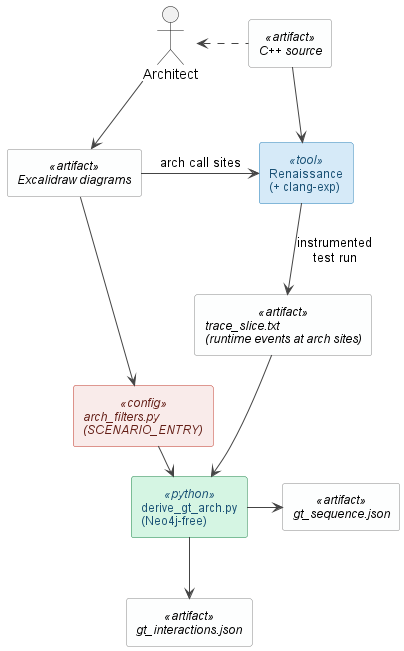
\includegraphics[width=0.7\textwidth]{figures/gt-derivation_v1.png}
\caption{Ground-truth derivation pipeline. An architect manually
  inspects the \Cpp\ source and draws Excalidraw structural and
  sequence diagrams for each scenario
  (\cref{sec:appendix-groundtruth}). These diagrams serve two roles:
  they identify the architecture-level call sites passed to Renaissance
  and \texttt{clang-exp} for guided instrumentation, and they define
  the \texttt{SCENARIO\_ENTRY} entry-point and \texttt{REACHABILITY}
  component-pair filters encoded in \texttt{arch\_filters.py}. The
  instrumented test run produces \texttt{trace\_slice.txt};
  \texttt{derive\_gt\_arch.py} then applies both filters and
  deduplicates to \texttt{gt\_interactions.json} and
  \texttt{gt\_sequence.json}.}
\label{fig:gt-derivation}
\end{figure}

Ground-truth construction begins with manual code inspection. The
architect reads the \Cpp\ source for each scenario, identifies the
cross-component call sites at the architectural boundary, and draws
structural and sequence diagrams in Excalidraw
(\cref{sec:appendix-groundtruth}). These hand-drawn diagrams are the
primary reference artefact; they are not derived from any pipeline
output.

The Excalidraw diagrams feed two downstream artefacts. First, the
identified call sites are passed to Renaissance and \texttt{clang-exp}
to configure guided instrumentation, so probes are placed exactly at
the architecture-level boundaries visible in the diagrams. Second, the
component pairs and entry-point functions visible in the diagrams are
encoded as filters in \texttt{arch\_filters.py}: a
\texttt{REACHABILITY} component-pair allowlist and a
\texttt{SCENARIO\_ENTRY} entry-point set.

When the instrumented test is run, it emits
\texttt{trace\_slice.txt}. \texttt{derive\_gt\_arch.py} reads this
trace, applies both filters from \texttt{arch\_filters.py}, and
deduplicates to \texttt{gt\_interactions.json} and
\texttt{gt\_sequence.json}. The ground truth is therefore fully
determined by the architect's manual inspection: the same Excalidraw
diagrams that configure instrumentation also define the filtering
rules, making the derivation independent of the Neo4j-based reachability filter and directly traceable to the
hand-drawn reference.

\section{SysML v2 Generation}\label{sec:sysml-generation}

The final stage projects the reachability-filtered output,
\texttt{interactions.json}
and \texttt{sequence.json} (\cref{sec:evidence-synthesis}), into \sysml
textual notation, using the SysML v2 constructs described in
\cref{sec:sysml}. The \texttt{draw-sysml-structural-model} skill reads
\texttt{interactions.json}: each unique component becomes a \texttt{part
def}, each interaction it sends or receives becomes a typed port on that
part, and each \texttt{(source, target, interaction)} triple becomes a
\texttt{connect} statement between the corresponding client and server
ports. The \texttt{draw-sysml-sequence-model} skill reads
\texttt{sequence.json}: each unique component becomes a lifeline
(\texttt{part def}), and each step becomes an ordered, labelled
\texttt{SynchronousCall} between the corresponding lifelines, with the
step number preserving the execution order recorded by synthesis.

Component names are derived algorithmically from file paths, not from a
hardcoded mapping table, using a path-to-component resolution function
that handles \texttt{/src/}, \texttt{/include/}, \texttt{/extern/}, and
\texttt{/tests/} prefixes, CamelCase normalisation, and \texttt{Impl}
suffix stripping. This keeps the generator codebase-agnostic: the same
script produces meaningful lifeline names on CPSCore or any other source
tree following standard C++ project layout conventions.
